\documentclass[11pt]{article}
\usepackage[margin=1in]{geometry}
\usepackage{amsmath,amssymb,amsfonts,mathtools}
\usepackage{booktabs,multirow,array,tabularx}
\usepackage{graphicx}
\usepackage{tikz}
\usepackage{pgfplots}
\pgfplotsset{compat=1.17}
\title{Plot Sample 2}
\author{Dataset-expansion sample}
\date{}
\begin{document}
\maketitle
\section{Visualization}
The figure below is a TikZ/pgfplots drawing drawn from a source-backed image-to-LaTeX benchmark.

\begin{figure}[htbp]
\centering
\scalebox{1}{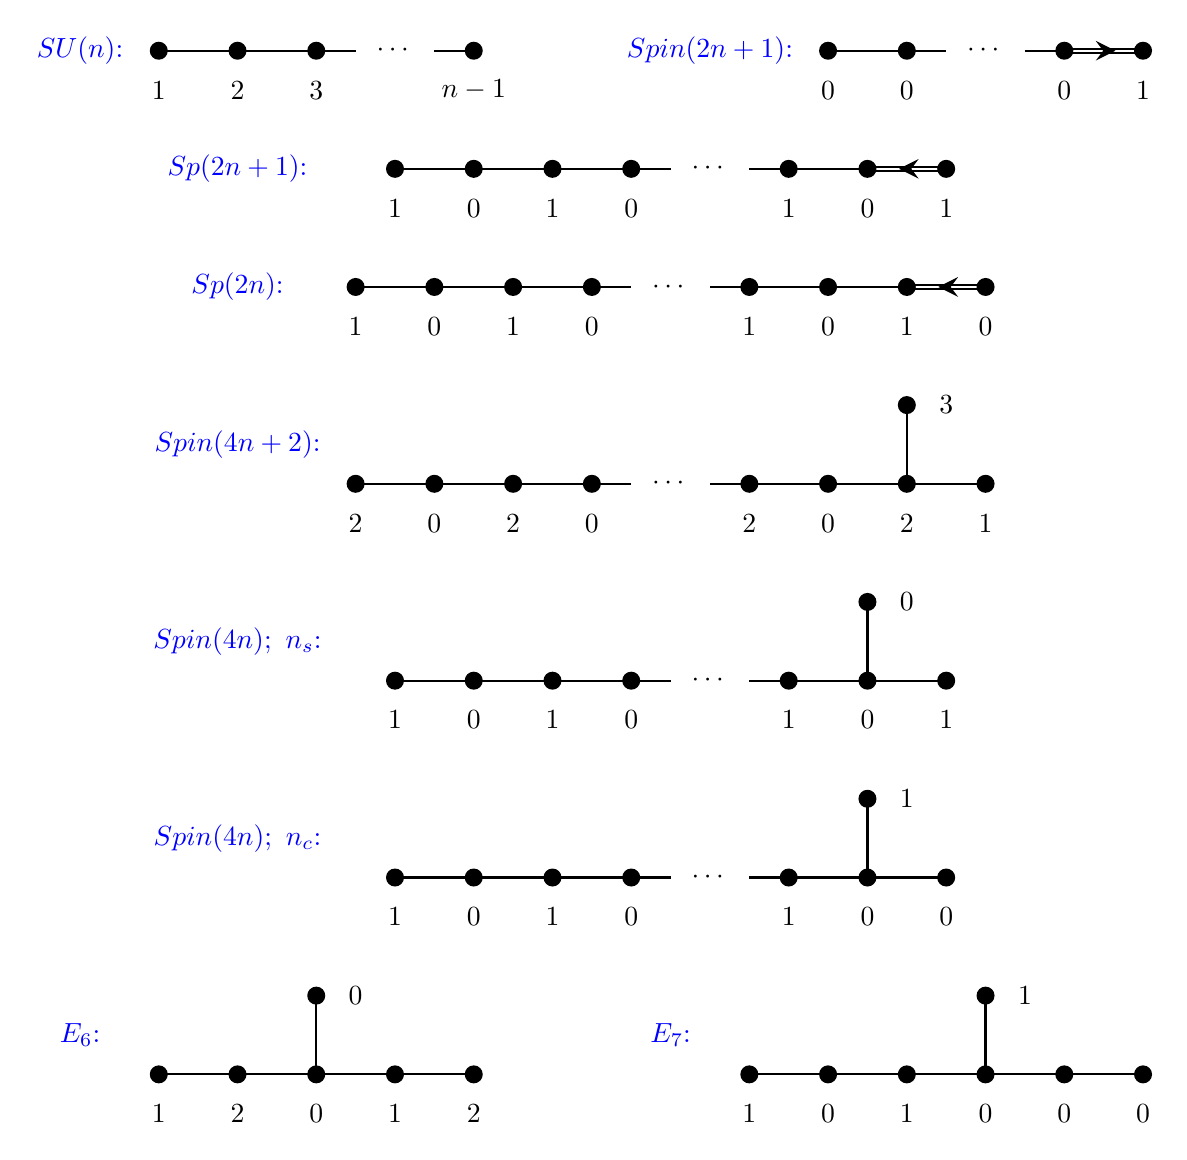
\begin{tikzpicture}
\draw [thick](-2,0) -- (0.5,0);
\draw [thick,fill=black] (-2,0) ellipse (0.1 and 0.1);
\draw [thick,fill=black] (-1,0) ellipse (0.1 and 0.1);
\draw [thick,fill=black] (0,0) ellipse (0.1 and 0.1);
\node at (1,0) {$\cdots$};
\draw [thick](1.5,0) -- (2,0);
\draw [thick,fill=black] (2,0) ellipse (0.1 and 0.1);
\node at (-2,-0.5) {1};
\node at (-1,-0.5) {2};
\node at (0,-0.5) {3};
\node at (2,-0.5) {$n-1$};
\node[blue] at (-3,0) {{$SU(n)$}:};
\begin{scope}
[shift={(8.5,0)}]
\draw [thick,double](1,0) -- (2,0);
\draw [ultra thick,double,-stealth](1.5,0) -- (1.65,0);
\draw [thick](-2,0) -- (-0.5,0);
\draw [thick,fill=black] (-2,0) ellipse (0.1 and 0.1);
\draw [thick,fill=black] (-1,0) ellipse (0.1 and 0.1);
\draw [thick,fill=black] (1,0) ellipse (0.1 and 0.1);
\node at (0,0) {$\cdots$};
\draw [thick](0.5,0) -- (1,0);
\draw [thick,fill=black] (2,0) ellipse (0.1 and 0.1);
\node at (-2,-0.5) {0};
\node at (-1,-0.5) {0};
\node at (1,-0.5) {0};
\node at (2,-0.5) {1};
\node[blue] at (-3.5,0) {{$Spin(2n+1)$}:};
\end{scope}
\begin{scope}
[shift={(3,-1.5)}]
\draw [thick,double](4,0) -- (5,0);
\draw [ultra thick,double,stealth-](4.4,0) -- (4.55,0);
\draw [thick](-2,0) -- (1.5,0);
\draw [thick,fill=black] (-2,0) ellipse (0.1 and 0.1);
\draw [thick,fill=black] (-1,0) ellipse (0.1 and 0.1);
\draw [thick,fill=black] (0,0) ellipse (0.1 and 0.1);
\draw [thick,fill=black] (1,0) ellipse (0.1 and 0.1);
\draw [thick,fill=black] (3,0) ellipse (0.1 and 0.1);
\draw [thick,fill=black] (4,0) ellipse (0.1 and 0.1);
\node at (2,0) {$\cdots$};
\draw [thick](2.5,0) -- (4,0);
\draw [thick,fill=black] (5,0) ellipse (0.1 and 0.1);
\node at (-2,-0.5) {1};
\node at (-1,-0.5) {0};
\node at (0,-0.5) {1};
\node at (1,-0.5) {0};
\node at (3,-0.5) {1};
\node at (4,-0.5) {0};
\node at (5,-0.5) {1};
\node [blue]at (-4,0) {{$Sp(2n+1)$}:};
\end{scope}
\begin{scope}
[shift={(2.5,-3)}]
\draw [thick,double](5,0) -- (6,0);
\draw [ultra thick,double,stealth-](5.4,0) -- (5.55,0);
\draw [thick](-2,0) -- (1.5,0);
\draw [thick,fill=black] (-2,0) ellipse (0.1 and 0.1);
\draw [thick,fill=black] (-1,0) ellipse (0.1 and 0.1);
\draw [thick,fill=black] (0,0) ellipse (0.1 and 0.1);
\draw [thick,fill=black] (1,0) ellipse (0.1 and 0.1);
\draw [thick,fill=black] (3,0) ellipse (0.1 and 0.1);
\draw [thick,fill=black] (4,0) ellipse (0.1 and 0.1);
\draw [thick,fill=black] (5,0) ellipse (0.1 and 0.1);
\node at (2,0) {$\cdots$};
\draw [thick](2.5,0) -- (5,0);
\draw [thick,fill=black] (6,0) ellipse (0.1 and 0.1);
\node at (-2,-0.5) {1};
\node at (-1,-0.5) {0};
\node at (0,-0.5) {1};
\node at (1,-0.5) {0};
\node at (3,-0.5) {1};
\node at (4,-0.5) {0};
\node at (5,-0.5) {1};
\node at (6,-0.5) {0};
\node[blue] at (-3.5,0) {{$Sp(2n)$}:};
\end{scope}
\begin{scope}
[shift={(2.5,-5.5)}]
\draw [thick](5,1) -- (5,0);
\draw [thick](5,0) -- (6,0);
\draw [thick](-2,0) -- (1.5,0);
\draw [thick,fill=black] (-2,0) ellipse (0.1 and 0.1);
\draw [thick,fill=black] (-1,0) ellipse (0.1 and 0.1);
\draw [thick,fill=black] (0,0) ellipse (0.1 and 0.1);
\draw [thick,fill=black] (1,0) ellipse (0.1 and 0.1);
\draw [thick,fill=black] (4,0) ellipse (0.1 and 0.1);
\draw [thick,fill=black] (3,0) ellipse (0.1 and 0.1);
\draw [thick,fill=black] (5,0) ellipse (0.1 and 0.1);
\node at (2,0) {$\cdots$};
\draw [thick](2.5,0) -- (5,0);
\draw [thick,fill=black] (6,0) ellipse (0.1 and 0.1);
\draw [thick,fill=black] (5,1) ellipse (0.1 and 0.1);
\node at (-2,-0.5) {2};
\node at (-1,-0.5) {0};
\node at (0,-0.5) {2};
\node at (1,-0.5) {0};
\node at (4,-0.5) {0};
\node at (3,-0.5) {2};
\node at (5,-0.5) {2};
\node at (6,-0.5) {1};
\node at (5.5,1) {3};
\node[blue] at (-3.5,0.5) {{$Spin(4n+2)$}:};
\end{scope}
\begin{scope}
[shift={(3,-8)}]
\draw [thick](4,1) -- (4,0);
\draw [thick](4,0) -- (5,0);
\draw [thick](-2,0) -- (1.5,0);
\draw [thick,fill=black] (-2,0) ellipse (0.1 and 0.1);
\draw [thick,fill=black] (-1,0) ellipse (0.1 and 0.1);
\draw [thick,fill=black] (0,0) ellipse (0.1 and 0.1);
\draw [thick,fill=black] (1,0) ellipse (0.1 and 0.1);
\draw [thick,fill=black] (3,0) ellipse (0.1 and 0.1);
\draw [thick,fill=black] (4,0) ellipse (0.1 and 0.1);
\node at (2,0) {$\cdots$};
\draw [thick](2.5,0) -- (4,0);
\draw [thick,fill=black] (5,0) ellipse (0.1 and 0.1);
\draw [thick,fill=black] (4,1) ellipse (0.1 and 0.1);
\node at (-2,-0.5) {1};
\node at (-1,-0.5) {0};
\node at (0,-0.5) {1};
\node at (1,-0.5) {0};
\node at (3,-0.5) {1};
\node at (4,-0.5) {0};
\node at (5,-0.5) {1};
\node at (4.5,1) {0};
\node[blue] at (-4,0.5) {{$Spin(4n);~n_s$}:};
\end{scope}
\begin{scope}
[shift={(3,-10.5)}]
\draw [thick](4,1) -- (4,0);
\draw [thick](4,0) -- (5,0);
\draw [thick](-2,0) -- (1.5,0);
\draw [thick,fill=black] (-2,0) ellipse (0.1 and 0.1);
\draw [thick,fill=black] (-1,0) ellipse (0.1 and 0.1);
\draw [thick,fill=black] (0,0) ellipse (0.1 and 0.1);
\draw [thick,fill=black] (1,0) ellipse (0.1 and 0.1);
\draw [thick,fill=black] (3,0) ellipse (0.1 and 0.1);
\draw [thick,fill=black] (4,0) ellipse (0.1 and 0.1);
\node at (2,0) {$\cdots$};
\draw [thick](2.5,0) -- (4,0);
\draw [thick,fill=black] (5,0) ellipse (0.1 and 0.1);
\draw [thick,fill=black] (4,1) ellipse (0.1 and 0.1);
\node at (-2,-0.5) {1};
\node at (-1,-0.5) {0};
\node at (0,-0.5) {1};
\node at (1,-0.5) {0};
\node at (3,-0.5) {1};
\node at (4,-0.5) {0};
\node at (5,-0.5) {0};
\node at (4.5,1) {1};
\node[blue] at (-4,0.5) {{$Spin(4n);~n_c$}:};
\end{scope}
\begin{scope}
[shift={(0,-13)}]
\draw [thick](0,1) -- (0,0);
\draw [thick](-2,0) -- (2,0);
\draw [thick,fill=black] (-2,0) ellipse (0.1 and 0.1);
\draw [thick,fill=black] (-1,0) ellipse (0.1 and 0.1);
\draw [thick,fill=black] (0,0) ellipse (0.1 and 0.1);
\draw [thick,fill=black] (1,0) ellipse (0.1 and 0.1);
\draw [thick,fill=black] (2,0) ellipse (0.1 and 0.1);
\draw [thick,fill=black] (0,1) ellipse (0.1 and 0.1);
\node at (-2,-0.5) {1};
\node at (-1,-0.5) {2};
\node at (0,-0.5) {0};
\node at (1,-0.5) {1};
\node at (2,-0.5) {2};
\node at (0.5,1) {0};
\node [blue] at (-3,0.5) {{$E_6$}:};
\end{scope}
\begin{scope}
[shift={(7.5,-13)}]
\draw [thick](1,1) -- (1,0);
\draw [thick](-2,0) -- (3,0);
\draw [thick,fill=black] (-2,0) ellipse (0.1 and 0.1);
\draw [thick,fill=black] (-1,0) ellipse (0.1 and 0.1);
\draw [thick,fill=black] (0,0) ellipse (0.1 and 0.1);
\draw [thick,fill=black] (1,0) ellipse (0.1 and 0.1);
\draw [thick,fill=black] (2,0) ellipse (0.1 and 0.1);
\draw [thick,fill=black] (3,0) ellipse (0.1 and 0.1);
\draw [thick,fill=black] (1,1) ellipse (0.1 and 0.1);
\node at (-2,-0.5) {1};
\node at (-1,-0.5) {0};
\node at (0,-0.5) {1};
\node at (1,-0.5) {0};
\node at (2,-0.5) {0};
\node at (3,-0.5) {0};
\node at (1.5,1) {1};
\node [blue] at (-3,0.5) {{$E_7$}:};
\end{scope}
\end{tikzpicture}}
\caption{Source-backed plot.}
\end{figure}

\end{document}
